% Document setup
\documentclass{article}
\usepackage{blindtext, multicol, comment, graphicx, caption, listings}
\usepackage[a4paper, margin=1.5cm]{geometry}
\graphicspath{ {./images/} }
\newenvironment{Figure}
  {\par\medskip\noindent\minipage{\linewidth}}
  {\endminipage\par\medskip}
\usepackage{amsmath}
\setlength{\columnsep}{1cm}
\usepackage{parskip}% http://ctan.org/pkg/parskip
\setlength{\parindent}{0pt}
\usepackage{float}


% \usepackage[demo]{graphicx}

% Caption stuff
\usepackage[format=plain, labelfont=it, textfont=it]{caption}

% Tables stuff
\usepackage{array}
\usepackage{booktabs} % makes nicer tables
\usepackage{multirow}
\newcommand{\rr}{\raggedright}
\newcommand{\rl}{\raggedleft}
\newcommand{\tn}{\tabularnewline}
\newcolumntype{x}[1]
{>{\raggedright}p{#1}}
\usepackage[singlelinecheck=false % <-- important
]{caption}

% Title
\title{\vspace{-0.5cm}
    \fontsize{14}{18} \selectfont {\textbf{Project 2 - Noise2Noise model from Scratch}}\\
    \fontsize{12}{18} {\selectfont EE-559 Deep Learning Course}
    }

\author{Naravich Chutisilp (341752), Veniamin Veselovsky (337188), Yasmin El Euch (250222)}
\date{May 2022}

\begin{document}
\maketitle

% Document
\begin{multicols}{2}
\section{Introduction}
In this project, the goal is to create a framework from the ground up that can be used to apply the Noise2Noise model to denoise a picture that lacks clean data. To do this, we will construct several modules such as the convolution module, activation functions, loss function, and optimizers while only using Pytorch library.

\section{Network Design}



The Module class is the basic foundation class around which the system revolves. A neural network as a whole may be thought of as an ordered collection of these modules. 
\begin{figure}[H] 
\centering 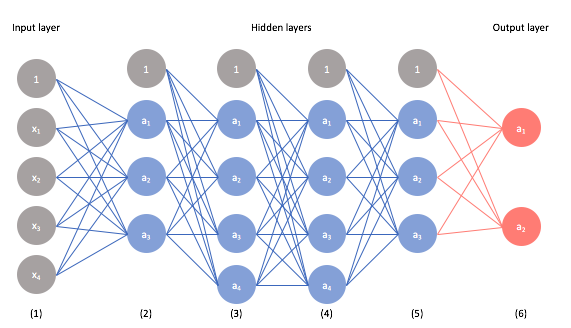
\includegraphics[width = 8.8cm]{pip.png}
\caption{Illustration of the implemented model}
\label{fig:model}
\end{figure}


\subsection{Sigmoid}
\begin{enumerate}
$
y = \sigma(x) = \frac{1}{1 + e^{-x}}
$
\\
\\
Wich will give gradient:
$
\frac{\partial {\mathcal{L}}}{\partial x} = 
    \frac{\partial {\mathcal{L}}}{\partial y} \sigma(x) (1 - \sigma(x))
$
\\
\end{enumerate}

\begin{equation}
\frac{\partial E}{{\partial L_{l-1}}} = (1 - {(\frac{e^{x}-e^{-x}}{e^{x}+e^{-x}})}^2) \cdot \frac{\partial E}{{\partial L_{l}}}
\label{eq:tanh_derivative}
\end{equation}

\subsection{ReLU}
\begin{enumerate}
Given a loss function $\mathcal{L}$, input $x$, output $y$ and activation function $f$, we are interested in $\frac{\partial{\mathcal{L}}}{\partial{x}}$ given that $y=f(x)$:

$$\frac{\partial{\mathcal{L}}}{\partial{x}}=\frac{\partial{\mathcal{L}}}{\partial{y}}\frac{\partial{y}}{\partial{x}}$$


\item \textbf{ReLU}: 
{$
\ y = \left\{
    \begin{array}{ll}
        \ x & \mbox{if } \ x > 0 \\
        \ 0 & \mbox{otherwise}
    \end{array}
\right.
$
\\
\\
the gradient is:
$
\ \frac{\partial {\mathcal{L}}}{\partial x} = \left\{
    \begin{array}{ll}
        \ \frac{\partial {\mathcal{L}}}{\partial y} & \mbox{if } \ x > 0 \\
        \ 0 & \mbox{otherwise}
    \end{array}
\right.
$
}
\\
\end{enumerate}
\subsection{Nearest Neighbour Upsampling}
Nearest Neighbour Interpolation determines the “nearest” neighbouring pixel, and assumes the intensity value of it.

\item \textbf{Forward}:
When a sequence of samples of a signal or other continuous function is upsampled, the result is a close approximation of the sequence that would have been produced if the signal had been sampled at a greater rate or density. The output is a repeated tensor which has the same shape as input but has a different size.
\item \textbf{Backward}:




\subsection{Padding}
parameters, forwardpass, backwardpass

\subsection{Upsampling}
parameters, forwardpass, backwardpass


\subsection{Conv2d}
parameters, forwardpass, backwardpass
Conv2d applies a 2D convolution over an input signal that is a tensor and consists of multiple planes.

\item \textbf{Forward}:

Computes the output of the convolution of the input with the kernel
\begin{itemize}
\begin{equation}
A_{o}^{(m)}=\sum_{k} W_{o k}^{(m)} * A_{k}^{(m-1)}+b_{o}^{(m)}
\end{equation}
With output shapes:


\begin{equation}

H_{\text {out }}=\left\lfloor\frac{H_{i n}+2 \times \text { padding }[0]-\text { dilation }[0] \times\text { (kernel_size-1) })}{\operatorname{stride}[0]}+1\right\rfloor

\end{equation}

\item \textbf{Backward}:

\begin{equation}
dA += \sum _{h=0} ^{n_H} \sum_{w=0} ^{n_W} W_c \times dZ_{hw} \tag{1}
\end{equation}
Where Wc is a filter and dZhw is a scalar equivalent to the cost gradient with respect to the conv layer Z output at the hth row and wth column (corresponding to the dot product taken at the ith stride left and jth stride down). When updating dA, we multiply the same filter Wc by a different dZ each time.  As a result, we sum the gradients of all the a slices when computing the backprop for dA.
\begin{equation}
dW_c  += \sum _{h=0} ^{n_H} \sum_{w=0} ^ {n_W} a_{slice} \times dZ_{hw}  \tag{2}
\end{equation}
Where  aslice corresponds to the slice used to generate the acitivation  Zij. Hence, we get the gradient for  W with respect to that slice. Since it is the same  W, we add up all such gradients to get  dW.


\begin{equation}
db = \sum_h \sum_w dZ_{hw} \tag{3}

\end{equation}
db is computed by summing  dZ. In this case, we are summing over all the gradients of the conv output (Z) with respect to the cost.



\subsection{Sequential}
This module, is the container  block for all neural networks of our framework.
\begin{itemize}
    \item \textbf{Instantiation Parameters:} \textit{modules} \\
    The Sequential organizes the modules - the $l$ (layers) and activation functions - passed as arguments in a sequential (ordered) manner.
    \item \textbf{Forward}($X \in \mathbb{R}^{dim_{in}}^{(1)} $): $\in \mathbb{R}^{dim_{out}}^{(l)}$ \\
   Iterates over all of the layers in ascending order, applying the current module's forward function on the preceding module's output.
   ($1$ to $l$)
    \item \textbf{Backward}($X \in \mathbb{R}^{dim_{out}}^{(l)} $): $\in \mathbb{R}^{dim_{in}}^{(1)}$ \\
    Iterates over all of the layers in reverse order, applying the current module's backward function on the preceding module's output. It gives the loss gradient with respect to the parameters.
\end{itemize}

\subsection{Model}
Sequential forwardpass, backwardpass

\subsection{Mean Square Error}
Mean Square Error is used to model how far off the estimation is. MSE is used as Criterion in the forward and backward pass as described in the table below.

\begin{table}[H]
    \centering
    \begin{tabular}{ | c | c | c | } 
        \hline
        Loss & Forward pass & Backward pass \\ [0.5ex]
        \hline
        MSE & $\frac{1}{n}\sum_{n=1}^{n} (y_i - \hat{y_i})^2$ & $2(Y - \hat{Y})$ \\ [1ex]
        \hline
    \end{tabular}
\end{table}

\subsection{Stochastic Gradient Descent Optimizer}
By updating the model's parameters in the opposite direction of the objective function's gradient, gradient descent is used to minimize the loss function L() with RD the model's parameters. On top of that, there various algorithms to optimize this approach in order to obtain fast convergence while avoiding getting locked in a local minimum. There are multiple gradient descents. The stochastic gradient descent offers a good compromise between accuracy and computation time.
\begin{itemize}
\item \textbf{SGD:} $$\theta^t+1 = \theta^{t} - \mu \nabla_\theta \mathcal{L}(\theta;x_j , y_j)$$ given $\mu$ the learning rate.
\item \textbf{SGD mini batch version:}
$$\theta^t+1 = \theta^{t} - \mu \nabla_\theta \mathcal{L}(\theta;x_{j,j+n} , y_{j,j+n})$$
\end{itemize}


\begin{table}[H]
    \centering
        \begin{tabular}{|l|l|}
        \hline
        \textbf{Sequential} & \textbf{Nout} \\ \hline
        conv1 (2x2 kernel, stride 2) & 48            \\ \hline
        relu1               & 48              \\ \hline
        conv2 (2x2 kernel, stride 2) & 96            \\ \hline
        relu2               &  96             \\ \hline
        upsampling3         & 48            \\ \hline
        relu3               &  48             \\ \hline
        upsampling4         & 3             \\ \hline
        activation          &  3             \\ \hline
    \end{tabular}
    \caption{The summary of the sequential model.}
    \label{tab:seq}
\end{table}

\section{Training}
Training

\section{Result}
Pending

\vspace{-8pt}
\begin{Figure}
 \centering
  \captionsetup{justification=centering}
 \includegraphics[width=\textwidth]{images/frog.jpg}
 \captionof{figure}{Example of Figure}
 \label{fig:example}
\end{Figure}

\section{Conclusion}
Conclusion


\bibliographystyle{IEEEtran}
\bibliography{main}
1-Jeremy Jordan. 2022. Deep neural networks: preventing overfitting.. [online] Available at: https://www.jeremyjordan.me/deep-neural
-networks-preventing-overfitting/

\end{multicols}
\end{document}
